\documentclass[10pt]{article}
\usepackage[polish]{babel}
\usepackage[utf8]{inputenc}
\usepackage[T1]{fontenc}
\usepackage{amsmath}
\usepackage{amsfonts}
\usepackage{amssymb}
\usepackage[version=4]{mhchem}
\usepackage{stmaryrd}
\usepackage{graphicx}
\usepackage[export]{adjustbox}
\graphicspath{ {./images/} }

\title{LIGA MATEMATYCZNA \\
 LISTOPAD 2010 \\
 SZKOŁA PODSTAWOWA }

\author{}
\date{}


\begin{document}
\maketitle
\section*{ZADANIE 1.}
Jakie wymiary, będące liczbami całkowitymi, powinna mieć prostokątna kartka papieru o polu powierzchni \(112 \mathrm{~cm}^{2}\), aby można było z niej wyciąć jak najwięcej kwadratów o wymiarach całkowitych i różnych polach?

\section*{ZADANIE 2.}
Podziel kwadrat \(4 \times 4\) przedstawiony na rysunku na cztery jednakowe części tak, aby każda litera była w innej części.\\
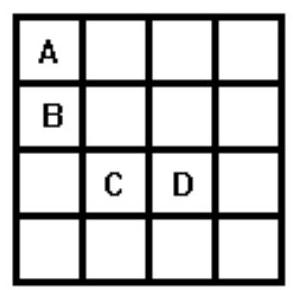
\includegraphics[max width=\textwidth, center]{2024_11_21_75ffe54ddbccdee3aceag-1(1)}

\section*{ZADANIE 3.}
W klasie IV b jest 29 uczniów. 18 uczniów ma brata, 17 uczniów ma siostrę. Tylko Zosia, Michał i Tomek nie mają żadnego rodzeństwa. Ilu uczniów ma brata i siostrę? (Żaden z uczniów nie ma więcej niż dwie osoby rodzeństwa.)

\section*{ZADANIE 4.}
Ala, Ela, Jola, Ola, Tola i Ula mieszkają w czteropiętrowym bloku. Ala mieszka wyżej niż Ela, ale niżej niż Jola. Ola i Tola mieszkają niżej niż Ula. Ola mieszka wyżej niż Ala, a Tola wyżej niż Jola. Która z dziewczynek mieszka na pierwszym piętrze?

\section*{ZADANIE 5.}
Uzupełnij puste kratki liczbami w taki sposób, aby suma każdej czwórki kolejnych liczb była równa 20.\\
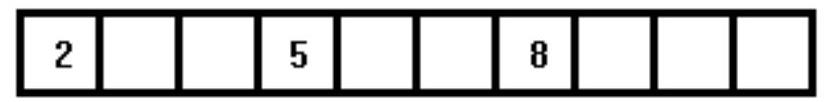
\includegraphics[max width=\textwidth, center]{2024_11_21_75ffe54ddbccdee3aceag-1}


\end{document}